\documentclass[11pt,a4paper]{article}
\usepackage{enumitem,amssymb,graphicx,epstopdf,hyperref,authblk}
\usepackage[T1]{fontenc}
\usepackage[utf8]{inputenc}

\begin{document}

\title{Introduction to Micro-controllers}
\date{\today} 
\author{Andres LaRosa}
\author{Bret Comnes}
\affil{Portland State University}
\maketitle

\section{Introduction} % (fold)
\label{sec:introduction}

Micro controllers are small computers designed to go where desktop computers dare not go.  They come in all shapes, sizes, and layouts.  Usually, they are quite small and use less power than traditional computers.  Typically they are deployed in an `appliances' and serve an unmodifiable dedicated purpose, such as keeping track of what spin cycle your washing machine is on, or how much time is left before it should turn off your microwave oven.  Make no mistake however, these are general purpose computers.  The other major difference between a microcontroller and desktop computer is that they they come with an array of analog and digital input and outputs. These can be used to read environmental data from sensors, talk to other computers or devices and electronically control other systems which provide environmental outputs such as a LCD screen, mechanical switch or servo motor.  \cite{wpmicro}

Getting started with microcontroller can be tedious process, as the require a number of supporting circuits, USB controllers, programmers, boot loaders, power supplies and chips, just to load your first program onto the microcontroller chip.  Often times you will start with a prototyping board, which takes a microcontroller and all the necessary tools to start working with it, and puts it on a single board, ready to start playing around with.

\subsection{Arduino} % (fold)
\label{sub:arduino}

\begin{quote}
\emph{``Arduino is a tool for making computers that can sense and control more of the physical world than your desktop computer. It's an open-source physical computing platform based on a simple microcontroller board, and a development environment for writing software for the board.''} -- \url{http://arduino.cc}
\end{quote}

This lab will be using the Arduino Leonardo Microcontroller\cite{leonardo}.  It is similar to the Arduino Uno\cite{uno}, with the major difference being that it uses SMT\cite{smt} instead of the older "thru-hole"\cite{th} technology.

Arduino drastically lowers the difficulty of getting started with a microcontroller, as it provides all the necessary tools to start making the microcontroller do interesting things without nearly all the setup of just a plain microcontroller.

Arduino is based around an 8-bit Atmel AVR microcontroller, and other good things like a boot loader for uploading programs, a USB controller for an easy source of power and connectivity to your computer as well as a barrel jack for non usb power sources.

It is programmed using a language that is based off of C++ and uses a fork of the Processing IDE.  Many arduino projects you will find will rely on programs running on your computer using Processing.\cite{processing}


% subsection arduino (end)

% section introduction (end)


\section{Getting Started} % (fold)
\label{sec:getting_started}

\subsection{Setting up your software} % (fold)

This lab is based off of the Arduino 1.0.3 software which can be downloaded for free from\cite{arduino-dl}.  Unlike other embedded systems development environments, the Arduino software is quick to download and set up, and has zero cost associated with the software which makes it a convenient to work with when your primary goal is to come up with a working prototype.

\newcommand\litem[1]{\item{\bfseries #1\\}}
\begin{enumerate}

\litem{Find a Computer} You are free to use your own laptop or one of the classroom computers.

\litem{Download and Launch the Arduino Software} Visit \url{http://arduino.cc/en/Main/Software} and downloaded the latest Arduino software\cite{arduino-dl}.  If you have decided to use your own Arduino, make sure you find the necessary USB drivers if you have a board that is older than the Uno.

\litem{Selecting the Correct Board} Once the IDE is open, navigate to the toolbar and select the board you are working with from \textbf{Toolbar $\rightarrow$ Tools $\rightarrow$ Board Arduino $\rightarrow$ Leonardo}.  Select a different board if you are using one.

\litem{Selecting a Serial Port}  This step varies from system to system.
    \begin{figure}[htbp]
        \centering
            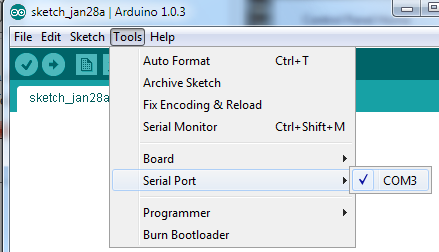
\includegraphics[height=3in]{figures/port-windows.png}
            
            
            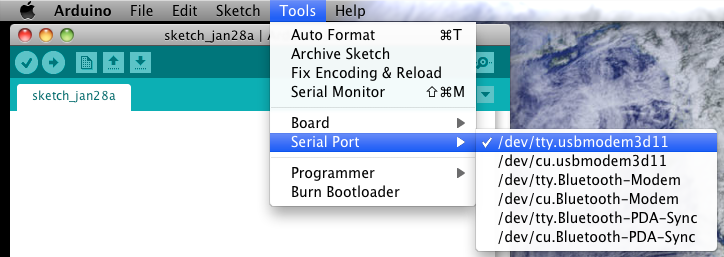
\includegraphics[height=2in]{figures/port-osx.png}
        \caption{Port Selection in Windows and OS X}
        \label{fig:figures_port}
    \end{figure}
    \newcommand\slitem[1]{\item{\bfseries #1\\}}
    \begin{enumerate}
        \slitem{Windows}
        Select \textbf{Toolbar $\rightarrow$ Tools $\rightarrow$ Serial Port $\rightarrow$ COM3} where COM3 is the serial port that has been assigned to your Arduino by windows.  You should only have one port available.
        
        
        \slitem{OS X}
        Select \textbf{Toolbar $\rightarrow$ Tools $\rightarrow$ Serial Port $\rightarrow$ /dev/tty.usbmodem3d11} where COM3 is the serial port that has been assigned to your Arduino by windows.  You should only have one port available.
    \end{enumerate}

\litem{Uploading your first program}
    Navigate to \textbf{Toolbar $\rightarrow$ File $\rightarrow$ Examples $\rightarrow$ 01. Basics $\rightarrow$ Blink}.  Press the verify button.  It should compile the sketch and return a `Done compiling' message.  If you get an error, something went wrong.
    \begin{figure}[htbp]
        \centering
            
\includegraphics{figures/verify.png}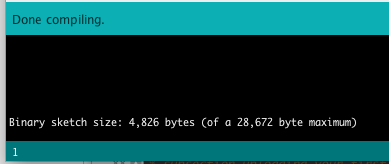
\includegraphics{figures/compile.png}
        \caption{Verify Button (Left) Compile Success Message (Right)}
        \label{fig:figures_verify}
    \end{figure}
    If that completed, go ahead and upload the program to the board by pressing the upload button and it should provide a similar completion message.  The LEDs on the arduino will blink during the upload, but should settle down after a few seconds.  Once the program you uploaded is running, the LED labeled `L' should be slowly blinking.  This LED labeled `L' is wired to Pin 13 on the arduino, a digital pin with a resistor built in that so that LEDs can be added easily.  \textbf{Go ahead and add an LED between Pin 13 and GND}.  It should blink at the same rate as `L' pin.
\end{enumerate}

Congratulations!  You now have a working Arduino that is talking to the Arduino IDE.



% subsection setting_up_your_software (end)

% section getting_started (end)

\section{Programming Arduino} % (fold)
\label{sec:programming_arduino}

Small intro text

\subsection{Syntax Basics} % (fold)
\label{sub:syntax_basics}

% subsection syntax_basics (end)

\subsection{Inputs} % (fold)
\label{sub:inputs}

% subsection inputs (end)

\subsection{Outputs} % (fold)
\label{sub:available_hardware}

% subsection available_hardware (end)



% section programming_arduino (end)

\bibliography{references} 
\bibliographystyle{plain} \nocite{*}

\end{document}